\chapter{Implementation}
In this chapter I discuss implementation details of the project.
The work is split into four modules, what Isabelle calls \emph{theories}.
The first (\emph{Fresh}, \S\ref{sec:freshness}) deals with fresh names, the second (\emph{Permutation}, \S\ref{sec:permutations}) with permutations, and the third and fourth (\emph{PreSimplyTyped}, \S\ref{sec:raw-terms} and \emph{SimplyTyped}, \S\ref{sec:quotient-terms}) with \(\lambda\)-terms, before and after the quotient respectively.
All theories build upon Isabelle's standard library, called \emph{Main}.
A dependency graph is shown in Figure \ref{fig:dependencies}.
Results shown which have a corresponding theorem in the formalisation are marked as such, like this:
\setcounter{theorem}{-1}
\begin{theorem}[\ident{example-in-isabelle}]
The statement of the theorem.
\end{theorem}
\begin{proof}
A proof of the theorem.
\end{proof}

\begin{figure}
\centering
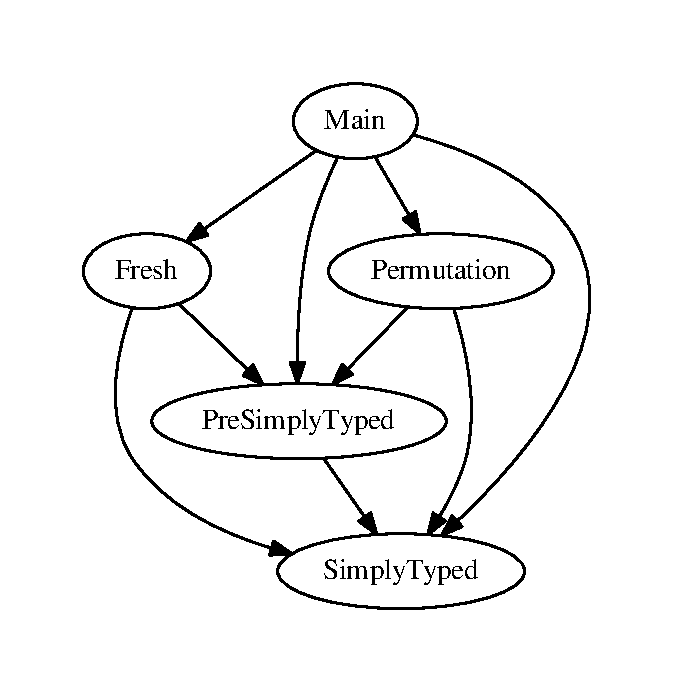
\includegraphics[width=.5\textwidth]{chapters/implementation/figures/dependencies}
\caption{A directed graph showing which of the theories depend on each other. \(A \to B\) shows that \(B\) depends upon results in \(A\).}
\label{fig:dependencies}
\end{figure}

\section{Freshness}
\label{sec:freshness}
I develop a theory of freshness, used later to obtain a fresh name for a given binder.
The implementation should accept a set of names \(S\), and produce an element not in \(S\).
In order to implement this interface, I used type classes~\cite{isabelle-typeclasses} to make a class for types that can produce a fresh element:

\begin{implementation}
\isacommand{class}\isamarkupfalse%
\ fresh\ =\isanewline
\ \ \isakeyword{fixes}\ fresh{\isacharunderscore}in\ {\isacharcolon}{\isacharcolon}\ {\isachardoublequoteopen}{\isacharprime}a\ set\ {\isasymRightarrow}\ {\isacharprime}a{\isachardoublequoteclose}\isanewline
\ \ \isakeyword{assumes}\ {\isachardoublequoteopen}finite\ S\ {\isasymLongrightarrow}\ fresh{\isacharunderscore}in\ S\ {\isasymnotin}\ S{\isachardoublequoteclose}
\end{implementation}

Note the pre-condition of a \emph{finite} \(S\): otherwise, useful implementations such as numbers or strings cannot conform to this interface.
To see this, consider (possibly-infinite) sets \(S\) of natural numbers.
Since \(S\) can be infinite, choose \(S\) to be \(\mathbb{N}\), the set of all natural numbers.
Now, if \(x\) is fresh in \(S\), \(x\) must be a natural number.
But since \(x \notin S\), \(x\) must also \emph{not} be a natural number, since \(S = \mathbb{N}\) --- a contradiction.

To extract executable code, there must be at least one implementation of freshness.
Unfortunately, not every implementation will suffice: for example, Isabelle allows the Hilbert indefinite description operator \(\epsilon\) inside definitions.
Hilbert's operator is a \emph{choice principle} --- the semantics of which are ``assuming that there is at least one \(x\) such that \(P(x)\), \(\epsilon x. P(x)\) chooses one such \(x\) (by no specific means) and returns \(x\)'' --- so
\[
\epsilon x. x \notin S
\]
would be a definition of freshness if there is such an \(x\) --- but this is not \emph{executable}, and code cannot be extracted from it.
Natural numbers are one possible implementation: to make a fresh natural number from a finite set \(S\), take the largest element of the set (or 0), then add 1 to it.

\begin{implementation}
\isacommand{instantiation}\isamarkupfalse%
\ nat\ {\isacharcolon}{\isacharcolon}\ fresh\isanewline
\isakeyword{begin}\isanewline
\ \ \isacommand{definition}\isamarkupfalse%
\ fresh{\isacharunderscore}in{\isacharunderscore}nat\ {\isacharcolon}{\isacharcolon}\ {\isachardoublequoteopen}nat\ set\ {\isasymRightarrow}\ nat{\isachardoublequoteclose}\ \isakeyword{where}\isanewline
\ \ \ \ {\isacharbrackleft}code{\isacharbrackright}{\isacharcolon}\ {\isachardoublequoteopen}fresh{\isacharunderscore}in{\isacharunderscore}nat\ S\ {\isasymequiv}\ {\isacharparenleft}if\ Set{\isachardot}is{\isacharunderscore}empty\ S\ then\ {\isadigit{0}}\ else\ Max\ S\ {\isacharplus}\ {\isadigit{1}}{\isacharparenright}{\isachardoublequoteclose}
\end{implementation}

The \texttt{code} tag indicates code to be extracted later.
The above also generates a proof obligation to show the implementation satisfies the freshness specification.

\begin{lemma}
For any finite set \(S\) of natural numbers, the procedure given produces an \(n\) such that \(n \notin S\).
\end{lemma}
\begin{proof}
\(S\) is either the empty set, or it is not.
If \(S\) is empty, 0 is produced as fresh in \(S\), and clearly \(0 \notin S\).
If \(S\) is non-empty, then \(n'\) is produced such that \(n'\) is larger than the largest element of \(S\), \(n\).
Suppose for contradiction that \(n'\) were in \(S\).
Then \(n'\) would be the largest element of \(S\), not \(n\).
Hence \(n'\) must not be in \(S\).
\end{proof}

\section{Swappings and permutations}
\label{sec:permutations}
Finitely-supported permutations are used in the nominal definition (\S\ref{sec:nominal-intro}) of \(\alpha\)-equivalence.
I define permutations as sequences of swappings, permuting by swapping single variables at a time.
Multiple sequences can correspond to the same permutation, so simple equality here will not suffice: permutations are ``equal'' iff they have the same effect on all inputs.
This is another use for quotient types: by identifying equivalent permutations, a new type can be made that does not make this distinction.
Therefore, I define \emph{pre-permutations}, then \emph{permutations}.
Here, I use type synonyms for the definition of the permutation type:

\begin{implementation}
\isacommand{type{\isacharunderscore}synonym}\isamarkupfalse%
\ {\isacharprime}a\ swp\ =\ {\isachardoublequoteopen}{\isacharprime}a\ {\isasymtimes}\ {\isacharprime}a{\isachardoublequoteclose}\isanewline
\isacommand{type{\isacharunderscore}synonym}\isamarkupfalse%
\ {\isacharprime}a\ preprm\ =\ {\isachardoublequoteopen}{\isacharprime}a\ swp\ list{\isachardoublequoteclose}
\end{implementation}

\begin{definition}[\ident{preprm-apply}]
Application of pre-permutations to names, \(\pi \dollar x\), is defined recursively:
\begin{enumerate}
\item
\(\varepsilon \dollar x = x\)
\item
\(\wrap{\wrap{a, b} :: \pi'} \cdot x = \wrap{a, b} \cdot \pi' \cdot x\), since \(\pi'\) is applied first, then \(\wrap{a, b}\).
\end{enumerate}
\end{definition}

\begin{implementation}
\isacommand{fun}\isamarkupfalse%
\ swp{\isacharunderscore}apply\ {\isacharcolon}{\isacharcolon}\ {\isachardoublequoteopen}{\isacharprime}a\ swp\ {\isasymRightarrow}\ {\isacharprime}a\ {\isasymRightarrow}\ {\isacharprime}a{\isachardoublequoteclose}\ \isakeyword{where}\isanewline
\ \ {\isachardoublequoteopen}swp{\isacharunderscore}apply\ {\isacharparenleft}a,\ b{\isacharparenright}\ x\ =\ {\isacharparenleft}if\ x\ =\ a\ then\ b\ else\ {\isacharparenleft}if\ x\ =\ b\ then\ a\ else\ x{\isacharparenright}{\isacharparenright}{\isachardoublequoteclose}\isanewline
\isanewline
\isacommand{fun}\isamarkupfalse%
\ preprm{\isacharunderscore}apply\ {\isacharcolon}{\isacharcolon}\ {\isachardoublequoteopen}{\isacharprime}a\ preprm\ {\isasymRightarrow}\ {\isacharprime}a\ {\isasymRightarrow}\ {\isacharprime}a{\isachardoublequoteclose}\ \isakeyword{where}\isanewline
\ \ {\isachardoublequoteopen}preprm{\isacharunderscore}apply\ {\isacharbrackleft}{\isacharbrackright}\ x\ =\ x{\isachardoublequoteclose}\isanewline
{\isacharbar}\ {\isachardoublequoteopen}preprm{\isacharunderscore}apply\ {\isacharparenleft}s\ {\isacharhash}\ ss{\isacharparenright}\ x\ {\isacharequal}\ swp{\isacharunderscore}apply\ s\ {\isacharparenleft}preprm{\isacharunderscore}apply\ ss\ x{\isacharparenright}{\isachardoublequoteclose}
\end{implementation}

The defined identity element is in fact identity:

\begin{lemma}[\ident{preprm-apply-id}]
\label{lemma:identity-application}
\(\varepsilon\) satisfies \(\varepsilon \dollar x = x\), for any \(x\).
\end{lemma}
\begin{proof}
By definition of application.
\end{proof}

In later proofs about \(\alpha\)-equivalence, I require that \(x = y \Longrightarrow \pi \dollar x = \pi \dollar y\) (which follows from identity), its inverse, \(x \neq y \Longrightarrow \pi \dollar x \neq \pi \dollar y\), and the converse, \(\pi \dollar x = \pi \dollar y \Longrightarrow x = y\).

\begin{lemma}[\ident{preprm-apply-unequal}]
\label{lemma:apply-unequal}
If \(x \neq y\), then \(\pi \dollar x \neq \pi \dollar y\)
\end{lemma}
\begin{proof}
By induction on \(\pi\).
The base case follows from Lemma \ref{lemma:identity-application}.
For the inductive step, suppose \(x' \neq y'\).
Then \([\wrap{a, b}] \dollar x' \neq [\wrap{a, b}] \dollar y'\), by cases on \(x'\) and \(y'\).
\end{proof}

\begin{lemma}[\ident{preprm-apply-injective}]
Application of permutations \(\pi\) is injective.
\end{lemma}
\begin{proof}
By induction on \(\pi\).
The base case follows by definition.
Using the inductive hypothesis, obtain \([(a, b)] \dollar \wrap{\pi' \dollar x} = [(a, b)] \dollar \wrap{\pi' \dollar y}\).
Then use the contrapositive of Lemma \ref{lemma:apply-unequal} to show that \(x = y\) using the inductive hypothesis.
\end{proof}

Some operations on pre-permutations are defined on the pre-permutations, then lifted over the equivalence relation.

\begin{definition}[\ident{preprm-compose}]
The composite pre-permutation \(\pi \diamond \sigma\) is \(\sigma\) appended to \(\pi\).
\end{definition}

\begin{lemma}[\ident{preprm-apply-composition}]
\label{lemma:apply-composition}
Application of \(\pi \diamond \sigma\) is equivalent to applying first \(\sigma\), then \(\pi\).
\end{lemma}
\begin{proof}
By induction on \(\pi\), both cases by definition.
\end{proof}

\begin{lemma}[\ident{preprm-unit-involution}]
\label{lemma:unit-involution}
Composition of \([\wrap{a, b}]\) with itself is equivalent to the identity element.
\end{lemma}
\begin{proof}
Consider whether \(x\), the variable the permutation is applied to, is \(a\), \(b\), or neither.
If it is \(a\) or \(b\), then swapping \(a\) to \(b\), then \(b\) to \(a\) (or vice-versa) produces the same \(x\).
If it is not, then the swapping has no effect.
\end{proof}

\begin{definition}[\ident{preprm-inv}]
The inverse of a permutation \(\pi\), \(\pi^{-1}\), is defined to be the reverse of \(\pi\).
\end{definition}

\begin{implementation}
\isacommand{definition}\isamarkupfalse%
\ preprm{\isacharunderscore}inv\ {\isacharcolon}{\isacharcolon}\ {\isachardoublequoteopen}{\isacharprime}a\ preprm\ {\isasymRightarrow}\ {\isacharprime}a\ preprm{\isachardoublequoteclose}\ \isakeyword{where}\isanewline
\ \ {\isachardoublequoteopen}preprm{\isacharunderscore}inv\ {\isasympi}\ {\isasymequiv}\ rev\ {\isasympi}{\isachardoublequoteclose}
\end{implementation}

It can be shown that this is the inverse operation:

\begin{lemma}[\ident{preprm-inv-involution}]
\label{lemma:inverse-involution}
For any \(\pi\) and \(x\), \(\pi^{-1} \dollar \pi \dollar x = x\), and vice-versa, \(\pi \dollar \pi^{-1} \dollar x = x\).
\end{lemma}
\begin{proof}
By induction on \(\pi\), with a trivial base case.
For the inductive step, assume that \(\pi'^{-1} \dollar \pi' \dollar x = x\) and try to show
\[
\wrap{[\wrap{a, b}] \diamond \pi'}^{-1} \dollar \wrap{[\wrap{a, b}] \diamond \pi'} \dollar x = x
\]

Note that
\[
\wrap{[\wrap{a, b}] \diamond \pi'}^{-1} = \pi'^{-1} \diamond [\wrap{a, b}]
\]
by definition.
Hence, using Lemmas \ref{lemma:apply-composition} and \ref{lemma:unit-involution} and the inductive hypothesis,
\begin{align*}
\wrap{[\wrap{a, b}] \diamond \pi'}^{-1} \dollar \wrap{\wrap{[\wrap{a, b}] \diamond \pi'} \dollar x}
&= \wrap{\pi'^{-1} \diamond [\wrap{a, b}]} \dollar \wrap{\wrap{[\wrap{a, b}] \diamond \pi'} \dollar x}\\
&= \pi'^{-1} \dollar \wrap{[\wrap{a, b}] \diamond [\wrap{a, b}]} \dollar \pi' \dollar x\\
&= \pi'^{-1} \dollar \wrap{\varepsilon} \dollar \pi' \dollar x\\
&= \pi'^{-1} \dollar \pi' \dollar x\\
&= x\\
\end{align*}
as required.
The alternative proposition follows from this and the fact that \(\wrap{\pi^{-1}}^{-1} = \pi\), given reversing a list is involutive.
\end{proof}

I define an extensional equivalence relation to relate equivalent permutations.

\begin{implementation}
\isacommand{definition}\isamarkupfalse%
\isanewline
\ \ preprm{\isacharunderscore}ext\ {\isacharcolon}{\isacharcolon}\ {\isachardoublequoteopen}{\isacharprime}a\ preprm\ {\isasymRightarrow}\ {\isacharprime}a\ preprm\ {\isasymRightarrow}\ bool{\isachardoublequoteclose}\isanewline
\ \ \isakeyword{where}\isanewline
\ \ {\isachardoublequoteopen}{\isasympi}\ =p\ {\isasymsigma}\ {\isasymequiv}\ {\isasymforall}x{\isachardot}\ preprm{\isacharunderscore}apply\ {\isasympi}\ x\ =\ preprm{\isacharunderscore}apply\ {\isasymsigma}\ x{\isachardoublequoteclose}
\end{implementation}

i.e. that \(\pi \equiv_p \sigma\) when for any \(x\) applying \(\pi\) and \(\sigma\) produces the same result.
This relation is an equivalence relation:

\begin{lemma}
\label{lemma:prm-equivalence}
\(\equiv_p\) is an equivalence relation.
\end{lemma}
\begin{proof}
Unfolding the definition of equivalence, \(\equiv_p\) is reflexive, symmetric, and transitive, and hence an equivalence relation.
\end{proof}

Several properties behave under equivalence as they would under equality.

\begin{lemma}[\ident{preprm-ext-compose-left}]
If \(\sigma \equiv_p \tau\), then \(\pi \diamond \sigma \equiv_p \pi \diamond \tau\).
\end{lemma}
\begin{lemma}[\ident{preprm-ext-compose-right}]
If \(\sigma \equiv_p \tau\), then \(\sigma \diamond \pi \equiv_p \tau \diamond \pi\).
\end{lemma}
\begin{proof}
Both of these follow from Lemma \ref{lemma:apply-composition}.
\end{proof}

\begin{lemma}[\ident{preprm-ext-uncompose}]
\label{lemma:uncompose}
If \(\pi \equiv_p \sigma\) and \(\pi \diamond \tau \equiv_p \sigma \diamond \rho\),
then \(\tau \equiv_p \rho\).
\end{lemma}
\begin{proof}
By assumption obtain \(\pi \diamond \tau \equiv_p \pi \diamond \rho\), then using the injectivity of permutation application, arrive at the result.
\end{proof}

\begin{lemma}[\ident{preprm-inv-ext}]
If \(\pi \equiv_p \sigma\), then \(\pi^{-1} \equiv_p \sigma^{-1}\).
\end{lemma}
\begin{proof}
Note that \(\wrap{\pi^{-1}}^{-1} \diamond \pi^{-1} \equiv_p \varepsilon\) and \(\wrap{\sigma^{-1}}^{-1} \diamond \sigma^{-1} \equiv_p \varepsilon\), using Lemma \ref{lemma:inverse-involution}.
Hence \(\pi \diamond \pi^{-1} \equiv_p \varepsilon\), and correspondingly for \(\sigma\).
From these obtain \(\pi \diamond \pi^{-1} \equiv_p \sigma \diamond \sigma^{-1}\), since \(\equiv_p\) is an equivalence relation.
Finally, derive the result by applying Lemma \ref{lemma:uncompose} and the assumptions.
\end{proof}

It is also expected that composition with an inverse produces identity.

\begin{lemma}[\ident{preprm-inv-compose}]
\label{lemma:group-inverse}
For any \(\pi\), \(\pi^{-1} \diamond \pi \equiv_p \varepsilon\).
\end{lemma}
\begin{proof}
Using Lemmas \ref{lemma:inverse-involution} and \ref{lemma:apply-composition}, this follows directly.
\end{proof}

The preceding theory can now be lifted into an extensional context with a quotient type.

\begin{implementation}
\isacommand{quotient{\isacharunderscore}type}\isamarkupfalse%
\ {\isacharprime}a\ prm\ =\ {\isachardoublequoteopen}{\isacharprime}a\ preprm{\isachardoublequoteclose}\ {\isacharslash}\ preprm{\isacharunderscore}ext\isanewline
%
\isatagproof
\isacommand{proof}\isamarkupfalse%
{\isacharparenleft}rule\ equivpI{\isacharparenright}\isanewline
\ \ \isacommand{show}\isamarkupfalse%
\ {\isachardoublequoteopen}reflp\ preprm{\isacharunderscore}ext{\isachardoublequoteclose}\ \isacommand{using}\isamarkupfalse%
\ preprm{\isacharunderscore}ext{\isacharunderscore}reflp\isacommand{{\isachardot}}\isamarkupfalse%
\isanewline
\ \ \isacommand{show}\isamarkupfalse%
\ {\isachardoublequoteopen}symp\ preprm{\isacharunderscore}ext{\isachardoublequoteclose}\ \isacommand{using}\isamarkupfalse%
\ preprm{\isacharunderscore}ext{\isacharunderscore}symp\isacommand{{\isachardot}}\isamarkupfalse%
\isanewline
\ \ \isacommand{show}\isamarkupfalse%
\ {\isachardoublequoteopen}transp\ preprm{\isacharunderscore}ext{\isachardoublequoteclose}\ \isacommand{using}\isamarkupfalse%
\ preprm{\isacharunderscore}ext{\isacharunderscore}transp\isacommand{{\isachardot}}\isamarkupfalse%
\isanewline
\isacommand{qed}\isamarkupfalse%
\endisatagproof
\end{implementation}

The quotient-type construction produces an obligation to show that \(\equiv_p\) is an equivalence (Lemma \ref{lemma:prm-equivalence}).
All work must now be lifted into the new equivalence.
Definitions are lifted like so:

\begin{implementation}
\isacommand{lift{\isacharunderscore}definition}\isamarkupfalse%
\ prm{\isacharunderscore}id\ {\isacharcolon}{\isacharcolon}\ {\isachardoublequoteopen}{\isacharprime}a\ prm{\isachardoublequoteclose}\ {\isacharparenleft}{\isachardoublequoteopen}{\isasymepsilon}{\isachardoublequoteclose}{\isacharparenright}\ \isakeyword{is}\ preprm{\isacharunderscore}id%
\end{implementation}

Lemmas as follows:

\begin{implementation}
\isacommand{lemma}\isamarkupfalse%
\ prm{\isacharunderscore}apply{\isacharunderscore}injective{\isacharcolon}\isanewline
\ \ \isakeyword{shows}\ {\isachardoublequoteopen}inj\ {\isacharparenleft}prm{\isacharunderscore}apply\ {\isasympi}{\isacharparenright}{\isachardoublequoteclose}\isanewline
%
\isadelimproof
%
\endisadelimproof
%
\isatagproof
\isacommand{by}\isamarkupfalse%
{\isacharparenleft}transfer,\ metis\ preprm{\isacharunderscore}apply{\isacharunderscore}injective{\isacharparenright}%
\endisatagproof
\end{implementation}

The set of permutations over a base set \(S\), \(P_S\) form a group \(\wrap{P_S, \circ}\): each element has an inverse, and \(\varepsilon\) is the identity element.
This is shown in the Isabelle source.
Other operations could be defined directly on the quotient type.

\begin{definition}[\ident{prm-set}]
The image of a set \(S\) under a permutation \(\pi\), \(\pi \image S\), is defined to be \(\{\pi \dollar x\ |\ x \in S\}\).
\end{definition}

This is the \emph{pointwise action} of \(\pi\) on \(S\), which allows for a permutation action on sets of names, and hence for a notion of equivariance on the free variables of a term.

\begin{implementation}
\isacommand{definition}\isamarkupfalse%
\ prm{\isacharunderscore}set\ {\isacharcolon}{\isacharcolon}\ {\isachardoublequoteopen}{\isacharprime}a\ prm\ {\isasymRightarrow}\ {\isacharprime}a\ set\ {\isasymRightarrow}\ {\isacharprime}a\ set{\isachardoublequoteclose}\ \isakeyword{where}\isanewline \ \ {\isachardoublequoteopen}prm{\isacharunderscore}set\ {\isasympi}\ S\ {\isasymequiv}\ image\ {\isacharparenleft}prm{\isacharunderscore}apply\ {\isasympi}{\isacharparenright}\ S{\isachardoublequoteclose}
\end{implementation}

\section{Raw \(\lambda\)-terms}
\label{sec:raw-terms}
Simple types \(\tau, \sigma, \ldots\) and \(\lambda\)-terms (uppercase variables) are defined as an Isabelle datatype, as described in \S\ref{sec:lambda-intro}.
I use natural numbers for a concrete variable type as they implement freshness, but any other type that satisfies freshness can be used.

\begin{implementation}
\isacommand{type{\isacharunderscore}synonym}\isamarkupfalse%
\ tvar\ =\ nat\isanewline
\isanewline
\isacommand{datatype}\isamarkupfalse%
\ type\ =\isanewline
\ \ TVar\ tvar\isanewline
{\isacharbar}\ TArr\ type\ type\isanewline
\isanewline
\isacommand{datatype}\isamarkupfalse%
\ {\isacharprime}a\ ptrm\ =\isanewline
\ \ PVar\ {\isacharprime}a\isanewline
{\isacharbar}\ PApp\ {\isachardoublequoteopen}{\isacharprime}a\ ptrm{\isachardoublequoteclose}\ {\isachardoublequoteopen}{\isacharprime}a\ ptrm{\isachardoublequoteclose}\isanewline
{\isacharbar}\ PFn\ {\isacharprime}a\ type\ {\isachardoublequoteopen}{\isacharprime}a\ ptrm{\isachardoublequoteclose}
\end{implementation}

The action of permutations on pre-terms, \(\pi \bullet X\) commutes with the structure of the term until the base case (i.e. variables or the name in a binder), so is expressed recursively.

\begin{implementation}
\isacommand{fun}\isamarkupfalse%
\ ptrm{\isacharunderscore}apply{\isacharunderscore}prm\ {\isacharcolon}{\isacharcolon}\ {\isachardoublequoteopen}{\isacharprime}a\ prm\ {\isasymRightarrow}\ {\isacharprime}a\ ptrm\ {\isasymRightarrow}\ {\isacharprime}a\ ptrm{\isachardoublequoteclose}\isanewline
\ \ {\isachardoublequoteopen}ptrm{\isacharunderscore}apply{\isacharunderscore}prm\ {\isasympi}\ {\isacharparenleft}PVar\ x{\isacharparenright}\ =\ PVar\ {\isacharparenleft}{\isasympi}\ {\isachardollar}\ x{\isacharparenright}{\isachardoublequoteclose}\isanewline
{\isacharbar}\ {\isachardoublequoteopen}ptrm{\isacharunderscore}apply{\isacharunderscore}prm\ {\isasympi}\ {\isacharparenleft}PApp\ A\ B{\isacharparenright}\ =\ PApp\isanewline
\ \ \ \ {\isacharparenleft}ptrm{\isacharunderscore}apply{\isacharunderscore}prm\ {\isasympi}\ A{\isacharparenright}\isanewline
\ \ \ \ {\isacharparenleft}ptrm{\isacharunderscore}apply{\isacharunderscore}prm\ {\isasympi}\ B{\isacharparenright}{\isachardoublequoteclose}\isanewline
{\isacharbar}\ {\isachardoublequoteopen}ptrm{\isacharunderscore}apply{\isacharunderscore}prm\ {\isasympi}\ {\isacharparenleft}PFn\ x\ T\ A{\isacharparenright}\ =\ PFn\ {\isacharparenleft}{\isasympi}\ {\isachardollar}\ x{\isacharparenright}\ T\ {\isacharparenleft}ptrm{\isacharunderscore}apply{\isacharunderscore}prm\ {\isasympi}\ A{\isacharparenright}{\isachardoublequoteclose}
\end{implementation}

I re-define results from \S\ref{sec:permutations} in the context of pre-terms by transcribing them.
For example, compare the following with corresponding lemmas about application of permutations.

\begin{implementation}
\isacommand{lemma}\isamarkupfalse%
\ ptrm{\isacharunderscore}prm{\isacharunderscore}apply{\isacharunderscore}id{\isacharcolon}\isanewline
\ \ \isakeyword{shows}\ {\isachardoublequoteopen}{\isasymepsilon}\ {\isasymbullet}\ X\ =\ X{\isachardoublequoteclose}\isanewline
\isatagproof
\isacommand{by}\isamarkupfalse%
{\isacharparenleft}induction\ X,\ simp{\isacharunderscore}all\ add{\isacharcolon}\ prm{\isacharunderscore}apply{\isacharunderscore}id{\isacharparenright}%
\endisatagproof
\isanewline
\isanewline
\isacommand{lemma}\isamarkupfalse%
\ ptrm{\isacharunderscore}prm{\isacharunderscore}apply{\isacharunderscore}compose{\isacharcolon}\isanewline
\ \ \isakeyword{shows}\ {\isachardoublequoteopen}{\isasympi}\ {\isasymbullet}\ {\isasymsigma}\ {\isasymbullet}\ X\ =\ {\isacharparenleft}{\isasympi}\ {\isasymdiamondop}\ {\isasymsigma}{\isacharparenright}\ {\isasymbullet}\ X{\isachardoublequoteclose}\isanewline
\isatagproof
\isacommand{by}\isamarkupfalse%
{\isacharparenleft}induction\ X,\ simp{\isacharunderscore}all\ add{\isacharcolon}\ prm{\isacharunderscore}apply{\isacharunderscore}composition{\isacharparenright}%
\endisatagproof
\end{implementation}

Free variables of a term can also be defined recursively.

\begin{implementation}
\isacommand{fun}\isamarkupfalse%
\ ptrm{\isacharunderscore}fvs\ {\isacharcolon}{\isacharcolon}\ {\isachardoublequoteopen}{\isacharprime}a\ ptrm\ {\isasymRightarrow}\ {\isacharprime}a\ set{\isachardoublequoteclose}\ \isakeyword{where}\isanewline
\ \ {\isachardoublequoteopen}ptrm{\isacharunderscore}fvs\ {\isacharparenleft}PVar\ x{\isacharparenright}\ {\isacharequal}\ {\isacharbraceleft}x{\isacharbraceright}{\isachardoublequoteclose}\isanewline
{\isacharbar}\ {\isachardoublequoteopen}ptrm{\isacharunderscore}fvs\ {\isacharparenleft}PApp\ A\ B{\isacharparenright}\ {\isacharequal}\ ptrm{\isacharunderscore}fvs\ A\ {\isasymunion}\ ptrm{\isacharunderscore}fvs\ B{\isachardoublequoteclose}\isanewline
{\isacharbar}\ {\isachardoublequoteopen}ptrm{\isacharunderscore}fvs\ {\isacharparenleft}PFn\ x\ {\isacharunderscore}\ A{\isacharparenright}\ {\isacharequal}\ ptrm{\isacharunderscore}fvs\ A\ {\isacharminus}\ {\isacharbraceleft}x{\isacharbraceright}{\isachardoublequoteclose}
\end{implementation}

Later, a set of names is frequently required to be finite, so that a fresh name can be generated.
To aid this, I show that the free variables of a pre-term is always a finite set.

\begin{lemma}[\texttt{ptrm-fvs-finite}]
The free variables of \(X\) form a finite set.
\end{lemma}
\begin{proof}
By induction on \(X\).
\end{proof}

This operation can also be shown equivariant using pointwise action, a property used later when working with the \(\alpha\)-equivalence of \(\lambda\)-terms:

\begin{lemma}[\ident{ptrm-prm-fvs}]
The free variables of \(\pi \bullet X\) are the image of \(\pi\) in the free variables of \(X\).
\end{lemma}
\begin{proof}
By induction on \(X\).
\begin{enumerate}
\item
For a variable \(x\), note that \(\pi \bullet x = \pi \dollar x\).
Then the proposition follows directly.
\item
Assume that \(\fvs\wrap{\pi \bullet A} = \pi \image \fvs(A)\), and similarly for \(B\).
Then the lemma holds for \(\wrap{A\ B}\):
\begin{align*}
\fvs\wrap{\pi \bullet \wrap{A\ B}}
&= \fvs\wrap{\wrap{\pi \bullet A}\ \wrap{\pi \bullet B}}\\
&= \fvs\wrap{\pi \bullet A} \cup \fvs\wrap{\pi \bullet A}\\
&= \pi \image \fvs(A) \cup \pi \image \fvs(B)\\
&= \pi \image \wrap{\fvs(A) \cup \fvs(B)}\\
&= \pi \image \fvs\wrap{A\ B}
\end{align*}
\item
Assume that \(\fvs\wrap{\pi \bullet A} = \pi \image \fvs(A)\).
Then finish as in the application case:
\begin{align*}
\fvs\wrap{\pi \bullet \lambda \wrap{x:T}.A} 
&= \fvs\wrap{\lambda \wrap{\pi \dollar x : T}. \wrap{\pi \bullet A}}\\
&= \fvs\wrap{\pi \bullet A} - \wrap{\pi \dollar x}\\
&= \pi \image \fvs(A) - \wrap{\pi \dollar x}\\
&= \pi \image \wrap{\fvs(A) - x}\\
&= \pi \image \wrap{\fvs\wrap{\lambda (x:T).A}}
\end{align*}
\end{enumerate}
\end{proof}

Isabelle generates a function called \texttt{size} with every datatype which reports the number of nodes in a given instance --- this corresponds to the formal definition of term size \(|M|\) described in \S\ref{sec:benchmarking}.
To use the size of a term (e.g. for induction), it is useful to show that size is equivariant, that \(|\pi \bullet M| = \pi \cdot |M| = |M|\).

\begin{lemma}[\ident{ptrm-size-prm}]
The size of a pre-term \(X\) is the same as the size of \(X\) under a permutation, \(\pi \bullet X\).
\end{lemma}
\begin{proof}
By induction on the structure of \(X\), then by definition of permutation application.
\end{proof}

\subsection{\(\alpha\)-equivalence}
Isabelle provides inductive definitions, so the nominal definition of \(\alpha\)-equivalence introduced in \S\ref{chap:preparation} is straightforward.
I used a slightly different formulation in which there are two cases for functions: one where the swapping variables are the same, and one when they are not.
This is equivalent, but makes for a shorter proof script.

\begin{implementation}
\isacommand{inductive}\isamarkupfalse%
\isanewline
\ \ ptrm{\isacharunderscore}alpha{\isacharunderscore}equiv\ {\isacharcolon}{\isacharcolon}\ {\isachardoublequoteopen}{\isacharprime}a\ ptrm\ {\isasymRightarrow}\ {\isacharprime}a\ ptrm\ {\isasymRightarrow}\ bool{\isachardoublequoteclose}\isanewline
\ \ \isakeyword{where}\isanewline
\ \ var{\isacharcolon}\ {\isachardoublequoteopen}{\isacharparenleft}PVar\ x{\isacharparenright}\ {\isasymapprox}\ {\isacharparenleft}PVar\ x{\isacharparenright}{\isachardoublequoteclose}\isanewline
{\isacharbar}\ app{\isacharcolon}\ {\isachardoublequoteopen}{\isasymlbrakk}A\ {\isasymapprox}\ B{\isacharsemicolon}\ C\ {\isasymapprox}\ D{\isasymrbrakk}\ {\isasymLongrightarrow}\ {\isacharparenleft}PApp\ A\ C{\isacharparenright}\ {\isasymapprox}\ {\isacharparenleft}PApp\ B\ D{\isacharparenright}{\isachardoublequoteclose}\isanewline
{\isacharbar}\ fn{\isadigit{1}}{\isacharcolon}\ {\isachardoublequoteopen}A\ {\isasymapprox}\ B\ {\isasymLongrightarrow}\ {\isacharparenleft}PFn\ x\ T\ A{\isacharparenright}\ {\isasymapprox}\ {\isacharparenleft}PFn\ x\ T\ B{\isacharparenright}{\isachardoublequoteclose}\isanewline
{\isacharbar}\ fn{\isadigit{2}}{\isacharcolon}\ {\isachardoublequoteopen}{\isasymlbrakk}a\ {\isasymnoteq}\ b{\isacharsemicolon}\ A\ {\isasymapprox}\ {\isacharbrackleft}a\ {\isasymleftrightarrow}\ b{\isacharbrackright}\ {\isasymbullet}\ B{\isacharsemicolon}\ a\ {\isasymnotin}\ ptrm{\isacharunderscore}fvs\ B{\isasymrbrakk}\isanewline
\ \ \ \ \ \ \ \ {\isasymLongrightarrow}\ {\isacharparenleft}PFn\ a\ T\ A{\isacharparenright}\ {\isasymapprox}\ {\isacharparenleft}PFn\ b\ T\ B{\isacharparenright}{\isachardoublequoteclose}
\end{implementation}

However, Isabelle does not provide eliminators by default, and these must be added manually.
Eliminators provide reasoning to ``go backwards'' from an inductive predicate, obtaining conditions which cause the truth of the predicate.
If \(\wrap{A\ C} \sim \wrap{B\ D}\), the only conclusion possible from the definition of \(\sim\) is that \(A \sim B\) and \(C \sim D\).

\begin{implementation}
\isacommand{inductive{\isacharunderscore}cases}\isamarkupfalse%
\ varE{\isacharcolon}\ \ {\isachardoublequoteopen}PVar\ x\ {\isasymapprox}\ Y{\isachardoublequoteclose}\isanewline
\isacommand{inductive{\isacharunderscore}cases}\isamarkupfalse%
\ appE{\isacharcolon}\ \ {\isachardoublequoteopen}PApp\ A\ B\ {\isasymapprox}\ Y{\isachardoublequoteclose}\isanewline
\isacommand{inductive{\isacharunderscore}cases}\isamarkupfalse%
\ fnE{\isacharcolon}\ \ \ {\isachardoublequoteopen}PFn\ x\ T\ A\ {\isasymapprox}\ Y{\isachardoublequoteclose}
\end{implementation}

These provide this style of reasoning, bound to labels as a theorem.
For instance \emph{varE} is effectively

\begin{implementation}
\isacommand{lemma}\isamarkupfalse%
\ varE\isanewline
\ \ \isakeyword{fixes}\ P\isanewline
\ \ \isakeyword{assumes}\ {\isachardoublequoteopen}PVar x\ {\isasymapprox}\ Y{\isachardoublequoteclose}\isanewline
\ \ \isakeyword{assumes}\ {\isachardoublequoteopen}Y = PVar x {\isasymLongrightarrow} P{\isachardoublequoteclose}\isanewline
\ \ \isakeyword{shows}\ {\isachardoublequoteopen}P{\isachardoublequoteclose}\isanewline
\isakeyword{proof}\isanewline
\ \ \ldots\isanewline
\isakeyword{qed}
\end{implementation}

A test of this relation is to show that free variables and permutation application are preserved under it, a property of \(\alpha\)-equivalence.

\begin{lemma}[\ident{ptrm-alpha-equiv-fvs}]
Assume \(X \sim Y\).
Then \(\fvs(X) = \fvs(Y)\).
\end{lemma}
\begin{proof}
By induction on the derivation of \(X \sim Y\).
\emph{var}, \emph{app}, and \emph{fn1} are easy.
For \emph{fn2}, assume:
\begin{itemize}
\item
\(a \neq b\)
\item
\(A \sim [a \swap b] \bullet B\)
\item
\(a \notin \fvs(B)\)
\item
the induction hypothesis, \(\fvs(A) = \fvs\wrap{[a \swap b] \bullet B}\)
\end{itemize}
Then, try and show \(\fvs\wrap{\lambda (a:T).A} = \fvs\wrap{\lambda (b:T).B}\).
\begin{align*}
\fvs\wrap{\lambda (a:T).A}
&= \fvs(A) - a\\
&= \fvs\wrap{[a \swap b] \bullet B} - a\\
&= \wrap{[a \swap b] \image \fvs(B)} - a\\
\end{align*}
Now the proof is stuck --- the proof will follow from arriving at the term \(\fvs(B) - b\), but simplifying will not arrive there.
Consider whether \(b\) is in the free variables of \(B\).
If it is, then \([a \swap b] \image \fvs(B) = \fvs(B) - {b} \cup {a}\), since \(a \notin \fvs(B)\), so
\begin{align*}
\wrap{[a \swap b] \image \fvs(B)} - a
&= \fvs(B) - {b} \cup {a} - a\\
&= \fvs(B) - b
\end{align*}
If it is not, then \([a \swap b]\) has no effect, so
\begin{align*}
\wrap{[a \swap b] \image \fvs(B)} - a
&= \fvs(B) - a\\
&= \fvs(B) = \fvs(B) - b
\end{align*}
Now
\begin{align*}
\fvs\wrap{\lambda (a:T).A}
&= \fvs(B) - b\\
&= \fvs\wrap{\lambda (b:T).B}
\end{align*}
\end{proof}

\begin{lemma}[\ident{ptrm-alpha-equiv-prm}]
\label{lemma:prm-equivalent}
Assume \(X \sim Y\).
Then \(\pi \bullet X \sim \pi \bullet Y\).
This shows that \(\alpha\)-equivalence is respected by permuting variable names.
\end{lemma}
\begin{proof}
By induction on the derivation of \(X \sim Y\).
Again \emph{var}, \emph{app}, and \emph{fn1} turn out to be easy.
For \emph{fn2}, assume as usual that \(a \neq b\), \(a \notin \fvs(B)\), and the induction hypothesis \(\pi \bullet A \sim \pi \bullet [a \swap b] \bullet B\).
Then, deduce from these the preconditions for \(\lambda (\pi \dollar a:T). \pi \bullet A \sim \lambda (\pi \dollar b:T). \pi \bullet B\), namely that
\begin{itemize}
\item
\(\pi \bullet a \neq \pi \bullet b\)
\item
\(\pi \dollar a \notin \fvs\wrap{\pi \bullet B}\)
\item
\(\pi \bullet A \sim [\pi \dollar a \swap \pi \dollar b] \bullet \pi \bullet B\)
\end{itemize}
Finally, see that both sides of the equivalence can be simplified to produce the result.
\end{proof}

I show that \(\sim\) is an equivalence relation.
Some specific results are needed first, which are presented informally:

\begin{lemma}[\ident{ptrm-swp-transfer}]
\label{lemma:transfer-swapping}
\([a \swap b] \bullet X \sim Y\) is equivalent to \(X \sim [a \swap b] \bullet Y\).
\end{lemma}
\begin{proof}
This is shown in both directions by permuting both sides by \([a \swap b]\), then using the fact that \([a \swap b] \diamond [a \swap b] = \varepsilon\).
\end{proof}

\begin{lemma}[\ident{ptrm-alpha-equiv-fvs-transfer}]
\label{lemma:transfer-freshness}
If \(a \notin \fvs(B)\), and \(A \sim [a \swap b] \bullet B\), then \(b \notin \fvs(A)\).
\end{lemma}
\begin{proof}
By a similar argument.
\end{proof}

These are used to argue reflexivity, symmetry, and transitivity.

\begin{lemma}[\ident{ptrm-alpha-equiv-reflexive}]
\(\sim\) is reflexive: that is, for all terms \(X\), \(X \sim X\).
\end{lemma}
\begin{proof}
By induction on the structure of \(X\).
\end{proof}

\begin{lemma}[\ident{ptrm-alpha-equiv-symmetric}]
\(\sim\) is symmetric, so for all terms \(X\), \(Y\), \(X \sim Y \Longrightarrow Y \sim X\).
\end{lemma}
\begin{proof}
By induction on the derivation of \(X \sim Y\).
As usual, \emph{fn2} is the difficult case.
It is given from the induction process that \(a \neq b\), \(A \sim [a \swap b] \bullet B\), \(a \notin \fvs(B)\), and the inductive hypothesis, \([a \swap b] \bullet B \sim A\).
From these and Lemmas \ref{lemma:transfer-swapping} and \ref{lemma:transfer-freshness}, deduce that \(b \neq a\), \(B \sim [b \swap a] \bullet A\), and \(b \notin \fvs(A)\).
These are the conditions for \(\lambda (b:T).B \sim \lambda (a:T).A\), which is the required result.
\end{proof}

\begin{lemma}[\ident{ptrm-alpha-equiv-transitive}]
\(\sim\) is transitive.
If \(X \sim Y\) and \(Y \sim Z\), then \(X \sim Z\).
\end{lemma}
\begin{proof}
By induction on the size of \(X\), then by cases on \(X\).
This generates the inductive hypothesis
\[
\forall K Y Z. \wrap{|K| < |X|, K \sim Y, Y \sim Z} \Longrightarrow K \sim Z
\]
If \(X\) is a variable, the result follows by deducing that \(Y\) and \(Z\) must also be variables (using the eliminators defined earlier), and that they must all be the same variable.
If \(X\) is instead an application, the inductive hypothesis can be used to show that both components of the application in \(X\) and \(Z\) are equivalent, and hence that \(X \sim Z\) by definition of \(\sim\).

Finally, if \(X\) is an abstraction, there are four cases to consider, depending on whether \emph{fn1} or \emph{fn2} is used to get from \(X\) to \(Y\), and again from \(Y\) to \(Z\).
The difficult case is when both relations are produced by \emph{fn2}.
This case can be further broken down when \(X\) and \(Z\) use the same variable in their binder --- suppose \(X = \lambda (x:T).A\), \(Y = \lambda (y:T).B\), and \(Z = \lambda (z:T). C\), then either \(x = z\) or \(x \neq z\).
If \(x = z\), then \(A \sim C\); since \(A \sim [x \swap y] \bullet B\) and \(B \sim [y \swap x] \bullet C\), \(A \sim [x \swap y] \bullet [y \swap x] \bullet C\), so \(A \sim C\) since the swappings cancel out.

However, if \(x \neq z\), \(X \sim Z\) has to be shown by \emph{fn2}.
Since both derivations were by \emph{fn2}, \(A \sim [x \swap y] \bullet [y \swap z] \bullet C\), but since \(x\), \(y\), and \(z\) are all now distinct it is possible to show (by definition of permutations) that \([x \swap y] \diamond [y \swap z] = [x \swap z]\), so \(A \sim [x \swap z] \bullet C\).
Also, \(x \notin \fvs(C)\) holds by noting that \(x \notin \fvs([y \swap z] \bullet C)\), then considering if \(z\) is in the free variables of \(C\).
If it is, then \(x \notin \fvs(C)\), since \(x \neq y \neq z\) and hence swapping \(z\) for \(y\) has no effect on whether \(x\) is in the free variables of the term or not.
If it is not, then the swapping has no effect, so \(x \notin \fvs(C)\) trivially.
Concluding, \(x \neq z\), \(A \sim [x \swap z] \bullet C\), and \(x \notin \fvs(C)\), so it follows that \(\lambda (x:T).A \sim \lambda (z:T).C\).
\end{proof}

\begin{theorem}
\(\sim\) is an equivalence relation.
\end{theorem}
\begin{proof}
Since \(\sim\) is reflexive, symmetric, and transitive, it is an equivalence relation.
\end{proof}

\subsection{Type inference algorithm}
\label{sec:type-inference}
I implement a type inference algorithm on the concrete syntax, which can then be lifted to terms.
The algorithm uses typing contexts, which are modelled as partial (i.e. total, but returning an option type) functions from names to types.

\begin{implementation}
\isacommand{type{\isacharunderscore}synonym}\isamarkupfalse%
\ {\isacharprime}a\ typing{\isacharunderscore}ctx\ {\isacharequal}\ {\isachardoublequoteopen}{\isacharprime}a\ {\isasymrightharpoonup}\ type{\isachardoublequoteclose}\isanewline
\isanewline
\isacommand{fun}\isamarkupfalse%
\ ptrm{\isacharunderscore}infer{\isacharunderscore}type\ {\isacharcolon}{\isacharcolon}\ {\isachardoublequoteopen}{\isacharprime}a\ typing{\isacharunderscore}ctx\ {\isasymRightarrow}\ {\isacharprime}a\ ptrm\ {\isasymRightarrow}\ type\ option{\isachardoublequoteclose}\ \isakeyword{where}\isanewline
\ \ {\isachardoublequoteopen}ptrm{\isacharunderscore}infer{\isacharunderscore}type\ {\isasymGamma}\ {\isacharparenleft}PVar\ x{\isacharparenright}\ {\isacharequal}\ {\isasymGamma}\ x{\isachardoublequoteclose}\isanewline
{\isacharbar}\ {\isachardoublequoteopen}ptrm{\isacharunderscore}infer{\isacharunderscore}type\ {\isasymGamma}\ {\isacharparenleft}PApp\ A\ B{\isacharparenright}\ {\isacharequal}\isanewline
\ \ \ \ {\isacharparenleft}case\ {\isacharparenleft}ptrm{\isacharunderscore}infer{\isacharunderscore}type\ {\isasymGamma}\ A{\isacharcomma}\ ptrm{\isacharunderscore}infer{\isacharunderscore}type\ {\isasymGamma}\ B{\isacharparenright}\ of\isanewline
\ \ \ \ \ \ {\isacharparenleft}Some\ {\isacharparenleft}TArr\ {\isasymtau}\ {\isasymsigma}{\isacharparenright}{\isacharcomma}\ Some\ {\isasymtau}{\isacharprime}{\isacharparenright}\ {\isasymRightarrow}\ {\isacharparenleft}if\ {\isasymtau}\ {\isacharequal}\ {\isasymtau}{\isacharprime}\ then\ Some\ {\isasymsigma}\ else\ None{\isacharparenright}\isanewline
\ \ \ \ {\isacharbar}\ {\isacharunderscore}\ {\isasymRightarrow}\ None{\isacharparenright}{\isachardoublequoteclose}\isanewline
{\isacharbar}\ {\isachardoublequoteopen}ptrm{\isacharunderscore}infer{\isacharunderscore}type\ {\isasymGamma}\ {\isacharparenleft}PFn\ x\ {\isasymtau}\ A{\isacharparenright}\ {\isacharequal}\isanewline
\ \ \ \ {\isacharparenleft}case\ ptrm{\isacharunderscore}infer{\isacharunderscore}type\ {\isacharparenleft}{\isasymGamma}{\isacharparenleft}x\ {\isasymmapsto}\ {\isasymtau}{\isacharparenright}{\isacharparenright}\ A\ of\isanewline
\ \ \ \ \ \ Some\ {\isasymsigma}\ {\isasymRightarrow}\ Some\ {\isacharparenleft}TArr\ {\isasymtau}\ {\isasymsigma}{\isacharparenright}\isanewline
\ \ \ \ {\isacharbar}\ None\ {\isasymRightarrow}\ None{\isacharparenright}{\isachardoublequoteclose}
\end{implementation}

To lift this definition, I show that it is invariant under \(\alpha\)-equivalence.
This is done with a lemma about swapping names in a typing context.

\begin{lemma}[\ident{ptrm-infer-type-swp}]
\label{lemma:infer-typing-swap}
Assume two names \(a\) and \(b\) are distinct, and \(b \notin \fvs(X)\).
Then
\[
\infertype\wrap{\Gamma\{a \mapsto \tau\}, X} = \infertype\wrap{\Gamma\{b \mapsto \tau\}, [a \swap b] \bullet X}
\]
\end{lemma}
\begin{proof}
By induction on the structure of \(X\).
\end{proof}

\begin{theorem}[\ident{ptrm-infer-type-alpha-equiv}]
The inference algorithm is invariant under equivalence.
If \(X \sim Y\), then for any context \(\Gamma\),
\[
\infertype\wrap{\Gamma, X} = \infertype\wrap{\Gamma, Y}
\]
\end{theorem}
\begin{proof}
By induction on the derivation of \(X \sim Y\).
All cases other than \emph{fn2} follow immediately by definition.
For \emph{fn2}, use the definition of the type inference algorithm and Lemma \ref{lemma:infer-typing-swap} to show that the function bodies have the same type \(\sigma\), then note that both \(X\) and \(Y\) then have inferred type \(\tau \to \sigma\).
\end{proof}

\section{\(\lambda\)-terms with \(\alpha\)-equivalence}
\label{sec:quotient-terms}
As before with permutations, pre-terms are lifted to terms using the quotient-type machinery.

\begin{implementation}
\isacommand{quotient{\isacharunderscore}type}\isamarkupfalse%
\ {\isacharprime}a\ trm\ {\isacharequal}\ {\isachardoublequoteopen}{\isacharprime}a\ ptrm{\isachardoublequoteclose}\ {\isacharslash}\ ptrm{\isacharunderscore}alpha{\isacharunderscore}equiv\isanewline
%
\isadelimproof
%
\endisadelimproof
%
\isatagproof
\isacommand{proof}\isamarkupfalse%
{\isacharparenleft}rule\ equivpI{\isacharparenright}\isanewline
\ \ \isacommand{show}\isamarkupfalse%
\ {\isachardoublequoteopen}reflp\ \ ptrm{\isacharunderscore}alpha{\isacharunderscore}equiv{\isachardoublequoteclose}\ \isacommand{using}\isamarkupfalse%
\ ptrm{\isacharunderscore}alpha{\isacharunderscore}equiv{\isacharunderscore}reflp\isacommand{{\isachardot}}\isamarkupfalse%
\isanewline
\ \ \isacommand{show}\isamarkupfalse%
\ {\isachardoublequoteopen}symp\ \ \ ptrm{\isacharunderscore}alpha{\isacharunderscore}equiv{\isachardoublequoteclose}\ \isacommand{using}\isamarkupfalse%
\ ptrm{\isacharunderscore}alpha{\isacharunderscore}equiv{\isacharunderscore}symp\isacommand{{\isachardot}}\isamarkupfalse%
\isanewline
\ \ \isacommand{show}\isamarkupfalse%
\ {\isachardoublequoteopen}transp\ ptrm{\isacharunderscore}alpha{\isacharunderscore}equiv{\isachardoublequoteclose}\ \isacommand{using}\isamarkupfalse%
\ ptrm{\isacharunderscore}alpha{\isacharunderscore}equiv{\isacharunderscore}transp\isacommand{{\isachardot}}\isamarkupfalse%
\isanewline
\isacommand{qed}\isamarkupfalse%
%
\endisatagproof
\end{implementation}

There is extra boilerplate required by the quotient, as equality rules don't necessarily hold.
First, every lifted constructor has to be shown to be not equal to every other constructor, of which the following is an indicative example.

\begin{implementation}
\isacommand{lemma}\isamarkupfalse%
\ var{\isacharunderscore}not{\isacharunderscore}app{\isacharcolon}\isanewline
\ \ \isakeyword{shows}\ {\isachardoublequoteopen}Var\ x\ {\isasymnoteq}\ App\ A\ B{\isachardoublequoteclose}\isanewline
%
\isadelimproof
%
\endisadelimproof
%
\isatagproof
\isacommand{proof}\isamarkupfalse%
{\isacharparenleft}transfer{\isacharparenright}\isanewline
\ \ \ldots\isanewline
\isacommand{qed}\isamarkupfalse%
%
\endisatagproof
\end{implementation}

Then, the ``obvious'' injective conclusions from equality don't necessarily hold either, and must be shown manually.
For example, suppose \(\wrap{A\ B} = \wrap{C\ D}\).
Conclude that \(A = C\) and \(B = D\) from this, but with the quotient type Isabelle cannot generate the result and it has to be shown manually.
Isabelle does not generate an induction principle for the new terms automatically, but I produce one by deferring to the concrete induction principle.

\begin{lemma}[\ident{trm-induct}]
Suppose \(P\) is a unary predicate on terms, and that for variables \(x\), \(P(x)\) holds, if \(P(A)\) and \(P(B)\) hold, then \(P\wrap{A\ B}\) also holds, and finally that if \(P(A)\) holds, then \(P\wrap{\lambda (x:T). A}\) also holds.
Then, for any \(M\), \(P(M)\).
\end{lemma}
\begin{proof}
Transfer the hypotheses to work on the concrete level, then show \(P\wrap{\textrm{Abs}(X)}\) by using the pre-term induction principle.
The lemma then follows by lifting this result.
\end{proof}

Similar principles are shown for case-analysis and induction on the size of a term.
\emph{Strong induction} allows assuming that \(x\) in a binder is fresh for a given set \(S\), which makes many proofs simpler and shorter --- a formalised version of Barendregt's convention.

\begin{lemma}[\ident{trm-strong-induct}]
\label{lemma:strong-induction}
Suppose now that \(P\) is a \emph{binary} predicate on pairs consisting of a set of names and a term.
The term is the object of induction, and \(S\) is a set of names to avoid when discussing binders.
Suppose that
\begin{enumerate}
\item
\(S\) is a finite set of names.
\item
\(P\wrap{S, x}\), for any variable \(x\).
\item
If \(P\wrap{S, A}\) and \(P\wrap{S, B}\), then \(P\wrap{S, \wrap{A\ B}}\).
\item
If \(x \notin S\) and \(P\wrap{S, A}\), then \(P\wrap{S, \wrap{\lambda (x:T). A}}\).
\end{enumerate}
Now for any term \(M\), \(P\wrap{S, M}\).
\end{lemma}
\begin{proof}
First, show a more general property: that for any permutation \(\pi\), \(P\wrap{S, \pi \cdot M}\).
This is argued by induction on \(M\), using the simple induction rule proved earlier.
The variable and application cases are by analogy with the simple induction, but the function binder needs special attention.
In the binding case, assume that \(P\wrap{S, \pi \cdot A}\) for any \(\pi\), and show that \(P\wrap{S, \pi \cdot \lambda (x:T).A}\).
To prove this, produce a new variable \(y\) (using the freshness implementation) that is fresh with respect to the union of \(S\), the free variables of \(\pi \cdot A\), and \(\pi \dollar z\).
Now for any \(B\), if \(P\wrap{S, B}\), then \(P\wrap{S, \lambda (y:T).B}\), using the assumptions --- in particular, \(P\wrap{S, \lambda (y:T). \wrap{[y \swap \pi \dollar x] \diamond \pi} \cdot A}\).

However, by using the \emph{fn2} rule, it can be shown that
\begin{align*}
\lambda (y:T). \wrap{[y \swap \pi \dollar x] \diamond \pi} \cdot A
&= \lambda (\pi \dollar x:T). \pi \cdot A\\
&= \pi \cdot \lambda (x:T). A
\end{align*}
And so \(P\wrap{S, \pi \cdot \lambda (x:T).A}\) holds for any \(\pi\).
Now that the stronger result is established, the original result can be shown by setting \(\pi = \varepsilon\).
\end{proof}

Further induction principles can be produced by combining the strong induction principle with proof by cases (``strong cases'') and proof by induction on the size of a term (``strong depth induction'').
Both follow immediately from the strong induction principle.

\begin{lemma}[\ident{trm-strong-cases}]
\label{lemma:strong-cases}
Suppose \(P\) and \(S\) are defined as in Lemma \ref{lemma:strong-induction}, but now consider a term \(M\) and suppose
\begin{enumerate}
\item
\(S\) is a finite set of names.
\item
If \(M = x\), or \(M = \wrap{A\ B}\), then \(P\wrap{S, M}\).
\item
If \(M = \lambda \wrap{x:T}. A\) and \(x \notin S\), then \(P\wrap{S, M}\).
\end{enumerate}
Then for any \(S\) and \(M\), \(P\wrap{S, M}\).
\end{lemma}

\begin{lemma}[\ident{trm-strong-depth-induct}]
Suppose \(P\) and \(S\) are defined as above.
Now, assume
\begin{enumerate}
\item
\(S\) is a finite set of names.
\item
\(P\wrap{S, x}\) holds for all \(x\).
\item
If \(P\wrap{S, K}\) holds for all \(K\) smaller than \(\wrap{A\ B}\), \(P\wrap{S, \wrap{A\ B}}\).
\item
If \(P\wrap{S, K}\) holds for all \(K\) smaller than \(\lambda \wrap{x:T}. A\), and \(x \notin S\), \(P\wrap{S, \lambda \wrap{x:T}.A}\).
\end{enumerate}
Then for any \(S\) and \(M\), \(P\wrap{S, M}\).
\end{lemma}

\subsection{Typing judgements}
\label{sec:typing-judgements}
An explicit typing relation is defined to ensure type inference is correct with respect to the relation.
Additionally, it is easier to argue that inductive definitions respect certain properties (e.g. preservation), then show that the algorithm is correct, than it is to argue directly about the algorithm.
The judgements presented in \S\ref{sec:type-intro} are encoded in Isabelle:

\begin{implementation}
\isacommand{inductive}\isamarkupfalse%
\ typing\ {\isacharcolon}{\isacharcolon}\ {\isachardoublequoteopen}{\isacharprime}a\ typing{\isacharunderscore}ctx\ {\isasymRightarrow}\ {\isacharprime}a\ trm\ {\isasymRightarrow}\ type\ {\isasymRightarrow}\ bool{\isachardoublequoteclose}\  \isakeyword{where}\isanewline
\ \ tvar{\isacharcolon}\ \ {\isachardoublequoteopen}{\isasymGamma}\ x\ {\isacharequal}\ Some\ {\isasymtau}\ {\isasymLongrightarrow}\ {\isasymGamma}\ {\isasymturnstile}\ Var\ x\ {\isacharcolon}\ {\isasymtau}{\isachardoublequoteclose}\isanewline
{\isacharbar}\ tapp{\isacharcolon}\ \ {\isachardoublequoteopen}{\isasymlbrakk}{\isasymGamma}\ {\isasymturnstile}\ f\ {\isacharcolon}\ {\isacharparenleft}TArr\ {\isasymtau}\ {\isasymsigma}{\isacharparenright}{\isacharsemicolon}\ {\isasymGamma}\ {\isasymturnstile}\ x\ {\isacharcolon}\ {\isasymtau}{\isasymrbrakk}\ {\isasymLongrightarrow}\ {\isasymGamma}\ {\isasymturnstile}\ App\ f\ x\ {\isacharcolon}\ {\isasymsigma}{\isachardoublequoteclose}\isanewline
{\isacharbar}\ tfn{\isacharcolon}\ \ \ {\isachardoublequoteopen}{\isasymGamma}{\isacharparenleft}x\ {\isasymmapsto}\ {\isasymtau}{\isacharparenright}\ {\isasymturnstile}\ A\ {\isacharcolon}\ {\isasymsigma}\ {\isasymLongrightarrow}\ {\isasymGamma}\ {\isasymturnstile}\ Fn\ x\ {\isasymtau}\ A\ {\isacharcolon}\ {\isacharparenleft}TArr\ {\isasymtau}\ {\isasymsigma}{\isacharparenright}{\isachardoublequoteclose}
\end{implementation}

The usual eliminators then need to be proved manually, as the quotient type adds complexity that Isabelle's inductive-cases command cannot currently process.
For example,

\begin{implementation}
\isacommand{lemma}\isamarkupfalse%
\ typing{\isacharunderscore}appE{\isacharcolon}\isanewline
\ \ \isakeyword{assumes}\ {\isachardoublequoteopen}{\isasymGamma}\ {\isasymturnstile}\ App\ A\ B\ {\isacharcolon}\ {\isasymsigma}{\isachardoublequoteclose}\isanewline
\ \ \isakeyword{shows}\ {\isachardoublequoteopen}{\isasymexists}{\isasymtau}{\isachardot}\ {\isacharparenleft}{\isasymGamma}\ {\isasymturnstile}\ A\ {\isacharcolon}\ {\isacharparenleft}TArr\ {\isasymtau}\ {\isasymsigma}{\isacharparenright}{\isacharparenright}\ {\isasymand}\ {\isacharparenleft}{\isasymGamma}\ {\isasymturnstile}\ B\ {\isacharcolon}\ {\isasymtau}{\isacharparenright}{\isachardoublequoteclose}
\end{implementation}

provides a mechanism for reasoning about the typing judgement of an application in reverse.
With these eliminators, I show the first property of the type system: weakening.

\begin{theorem}[\ident{typing-weaken}]
Assume that \(\Gamma \vdash M : \tau\), and pick \(y\) such that \(y \notin \fvs(M)\).
Then
\[\Gamma\{y \mapsto \sigma\} \vdash M : \tau\]
for any \(\sigma\) --- weakening the context with another variable \(y\) derives the same type, providing that \(y\) is fresh.
\end{theorem}
\begin{proof}
By induction on the derivation of the typing judgement.
\emph{tvar} and \emph{tapp} follow directly, but the presence of a binder in \emph{tfn} complicates matters.
By assumption, note \(y \notin \fvs\wrap{\lambda (x:\tau). A}\), so either \(y = x\) or \(y \notin \fvs(A)\).
In the first case, adding the \(x \mapsto \tau\) to the context overwrites the weakened context.
For the second, \(y \notin \fvs(A)\) can be combined with the induction hypothesis to show the result.
\end{proof}

\subsection{Substitution and \(\beta\)-reduction}
\label{sec:beta-reduction}
Some theorems about the type system of the calculus require \(\beta\)-reduction, which itself requires substitution to be defined first.
I define a substitution relation inductively, then show that the relation is a function, then define \(\beta\)-reduction in terms of it.
While it is possible to define substitution as a function directly, it has to be defined on pre-terms, then lifted, as Isabelle's function package does not support defining functions on equivalence classes.

\begin{implementation}
\isacommand{inductive}\isamarkupfalse%
\ substitutes\ {\isacharcolon}{\isacharcolon}\ {\isachardoublequoteopen}{\isacharprime}a\ trm\ {\isasymRightarrow}\ {\isacharprime}a\ {\isasymRightarrow}\ {\isacharprime}a\ trm\ {\isasymRightarrow}\ {\isacharprime}a\ trm\ {\isasymRightarrow}\ bool{\isachardoublequoteclose}\ \isakeyword{where}\isanewline
\ \ var{\isadigit{1}}{\isacharcolon}\ {\isachardoublequoteopen}x\ {\isacharequal}\ y\ {\isasymLongrightarrow}\ substitutes\ {\isacharparenleft}Var\ x{\isacharparenright}\ y\ M\ M{\isachardoublequoteclose}\isanewline
{\isacharbar}\ var{\isadigit{2}}{\isacharcolon}\ {\isachardoublequoteopen}x\ {\isasymnoteq}\ y\ {\isasymLongrightarrow}\ substitutes\ {\isacharparenleft}Var\ x{\isacharparenright}\ y\ M\ {\isacharparenleft}Var\ x{\isacharparenright}{\isachardoublequoteclose}\isanewline
{\isacharbar}\ app{\isacharcolon}\ \ {\isachardoublequoteopen}{\isasymlbrakk}substitutes\ A\ x\ M\ A{\isacharprime}{\isacharsemicolon}\ substitutes\ B\ x\ M\ B{\isacharprime}{\isasymrbrakk}\isanewline
\ \ \ \ \ \ {\isasymLongrightarrow}\ substitutes\ {\isacharparenleft}App\ A\ B{\isacharparenright}\ x\ M\ {\isacharparenleft}App\ A{\isacharprime}\ B{\isacharprime}{\isacharparenright}{\isachardoublequoteclose}\isanewline
{\isacharbar}\ fn{\isacharcolon}\ \ \ {\isachardoublequoteopen}{\isasymlbrakk}x\ {\isasymnoteq}\ y{\isacharsemicolon}\ y\ {\isasymnotin}\ fvs\ M{\isacharsemicolon}\ substitutes\ A\ x\ M\ A{\isacharprime}{\isasymrbrakk}\isanewline
\ \ \ \ \ \ {\isasymLongrightarrow} substitutes\ {\isacharparenleft}Fn\ y\ T\ A{\isacharparenright}\ x\ M\ {\isacharparenleft}Fn\ y\ T\ A{\isacharprime}{\isacharparenright}{\isachardoublequoteclose}
\end{implementation}

If a relation \(R\) is a function, it is both \emph{total} and \emph{single-valued}, so that \(R\) satisfies
\[
\forall a. \exists b. R(a, b)
\]
and
\[
\forall a, b, c. R(a, b) \wedge R(a, c) \Longrightarrow b = c
\]

\begin{lemma}[\ident{substitutes-total}]
\label{lemma:substitution-total}
The substitution relation is total: for any term \(A\), there is an \(A'\) which is the substitution of \(x\) for \(M\) in \(A\).
\end{lemma}
\begin{proof}
By strong induction on \(A\), avoiding both \(x\) and the free variables of \(M\).
For the variable case, consider whether the variable is equal to \(x\) or not, and use either the \emph{var1} or \emph{var2} rules accordingly.
Applications follow from the induction hypotheses.
Finally, for functions \(\lambda (y:T). B\), note that \(y \neq x\) and \(y \notin \fvs(M)\), by the strong induction hypothesis.
Hence the \emph{fn} rule applies.
\end{proof}

\begin{lemma}[\ident{substitutes-unique}]
\label{lemma:substitution-unique}
The substitution relation is unique: if \(B\) and \(C\) are both substitutions of \(x\) for \(M\) in \(A\), then \(B = C\).
\end{lemma}
\begin{proof}
By strong induction on \(A\), avoiding \(x\) and \(\fvs(M)\), then directly using eliminators.
\end{proof}

\begin{lemma}[\ident{substitutes-function}]
Substitution is a function.
\end{lemma}
\begin{proof}
Using Lemmas \ref{lemma:substitution-unique} and \ref{lemma:substitution-total}, by definition.
\end{proof}

Isabelle can produce a function from this result and the relation.
This is done using the definition description operator \(\iota\), which Isabelle calls ``THE'' --- this is like the indefinite description operator, but returns the \emph{only} such item.
Then, a series of simplification lemmas are provided to allow reasoning about the function.
While substitution is an executable algorithm, this definition is not exexecutable as there is no direct definition.
It may be possible to use Isabelle's code transformation with added user-defined properties to allow an extracted implementation (discussed later), but this is left as an extension.

\begin{implementation}
\isacommand{definition}\isamarkupfalse%
\ subst\ {\isacharcolon}{\isacharcolon}\ {\isachardoublequoteopen}{\isacharprime}a\ trm\ {\isasymRightarrow}\ {\isacharprime}a\ {\isasymRightarrow}\ {\isacharprime}a\ trm\ {\isasymRightarrow}\ {\isacharprime}a\ trm{\isachardoublequoteclose}\ {\isacharparenleft}{\isachardoublequoteopen}{\isacharunderscore}{\isacharbrackleft}{\isacharunderscore}\ {\isacharcolon}{\isacharcolon}{\isacharequal}\ {\isacharunderscore}{\isacharbrackright}{\isachardoublequoteclose}{\isacharparenright}\ \isakeyword{where}\isanewline
\ \ {\isachardoublequoteopen}subst\ A\ x\ M\ {\isasymequiv}\ {\isacharparenleft}THE\ X{\isachardot}\ substitutes\ A\ x\ M\ X{\isacharparenright}{\isachardoublequoteclose}
\end{implementation}

I showcase the strength of the strong induction principle (and hence the whole nominal approach) by showing \emph{Barendregt's substitution lemma}~\cite{lambda-overview}, which allows re-writing substitutions in a different order.
It is used to show the confluence property.

\begin{lemma}[\ident{barendregt}]
Assume that \(y \neq z\), and that \(y \notin \fvs(L)\).
Then
\[
M[y := N][z := L] = M[z := L][y := N[z := L]]
\]
\end{lemma}
\begin{proof}
By strong induction on \(M\), avoiding \(y\), \(z\), and the free variables of \(N\) and \(L\).
Normally, the proof proceeds by induction on \(M\), deals easily with the variable and application cases, then becomes concerned with details of name clashing in the binder case.
Consider \(M = \lambda x. A\).
At this point, substitution cannot necessarily be simplified as it may not be capture-avoiding.
However, using the strong induction principle, it is provided that \(x \neq y\), \(x \neq z\), and \(x\) is fresh for both \(N\) and \(L\).
Therefore, the proof follows by simplification directly:
\begin{align*}
\wrap{\lambda x. A}[y := N][z := L]
&= \lambda x. \wrap{A[y := N][z := L]}\\
&= \lambda x. \wrap{A[z := L][y := N[z := L]]}\\
&= \wrap{\lambda x. A}[z := L][y := N[z := L]]
\end{align*}
It can be seen here that by avoiding the names, and hence the problem, the proof is much simpler and the binder case follows directly.
\end{proof}

I show a result about the effect of substitution on typing, which is used while contracting a \(\beta\)-redex in the proof of type-preservation.
This lemma also exercises the strong depth-induction principle, combining avoiding name conflicts in the proof and also assuming that the result holds for any term smaller than the term currently under consideration.

\begin{lemma}[\ident{typing-subst}]
\label{lemma:typing-subst}
Assume that \(\Gamma \vdash N : \tau\), and also that \(\Gamma\{z \mapsto \tau\} \vdash M : \sigma\).
Then \(\Gamma \vdash M[z := N] : \sigma\).
\end{lemma}
\begin{proof}
By strong induction on the size of \(M\), avoiding \(z\) and \(\fvs(N)\).
The case of variables \(x\) follows by considering \(x = z\), and the application case follows from the inductive hypothesis.
For binders, the weakening result about the type system can be used to show that \(\Gamma\{x \mapsto T\} \vdash N : \tau\).
By assumption, \(\Gamma\{z \mapsto \tau\} \vdash \lambda (x:T).A : \sigma\), and hence there is a type \(\sigma'\) such that \(\sigma = T \to \sigma'\), and
\[
\Gamma\{z \mapsto \tau, x \mapsto T\} \vdash A : \sigma'
\]
Hence by the inductive hypotheses, \(\Gamma\{x \mapsto T\} \vdash A[z := N] : \sigma'\), then
\[
\Gamma \vdash \lambda (x:T). A[z := N] : \sigma
\]
The result follows by simplification.
\end{proof}

I used substitution to define single-step \(\beta\)-reduction:

\begin{implementation}
\isacommand{inductive}\isamarkupfalse%
\ beta{\isacharunderscore}reduction\ {\isacharcolon}{\isacharcolon}\ {\isachardoublequoteopen}{\isacharprime}a\ trm\ {\isasymRightarrow}\ {\isacharprime}a\ trm\ {\isasymRightarrow}\ bool{\isachardoublequoteclose}\ \isakeyword{where}\isanewline
\ \ beta{\isacharcolon}\ \ {\isachardoublequoteopen}{\isacharparenleft}App\ {\isacharparenleft}Fn\ x\ T\ A{\isacharparenright}\ M{\isacharparenright}\ {\isasymrightarrow}{\isasymbeta}\ {\isacharparenleft}A{\isacharbrackleft}x\ {\isacharcolon}{\isacharcolon}{\isacharequal}\ M{\isacharbrackright}{\isacharparenright}{\isachardoublequoteclose}\isanewline
{\isacharbar}\ app{\isadigit{1}}{\isacharcolon}\ \ {\isachardoublequoteopen}A\ {\isasymrightarrow}{\isasymbeta}\ A{\isacharprime}\ {\isasymLongrightarrow}\ {\isacharparenleft}App\ A\ B{\isacharparenright}\ {\isasymrightarrow}{\isasymbeta}\ {\isacharparenleft}App\ A{\isacharprime}\ B{\isacharparenright}{\isachardoublequoteclose}\isanewline
{\isacharbar}\ app{\isadigit{2}}{\isacharcolon}\ \ {\isachardoublequoteopen}B\ {\isasymrightarrow}{\isasymbeta}\ B{\isacharprime}\ {\isasymLongrightarrow}\ {\isacharparenleft}App\ A\ B{\isacharparenright}\ {\isasymrightarrow}{\isasymbeta}\ {\isacharparenleft}App\ A\ B{\isacharprime}{\isacharparenright}{\isachardoublequoteclose}\isanewline
{\isacharbar}\ fn{\isacharcolon}\ \ \ \ {\isachardoublequoteopen}A\ {\isasymrightarrow}{\isasymbeta}\ A{\isacharprime}\ {\isasymLongrightarrow}\ {\isacharparenleft}Fn\ x\ T\ A{\isacharparenright}\ {\isasymrightarrow}{\isasymbeta}\ {\isacharparenleft}Fn\ x\ T\ A{\isacharprime}{\isacharparenright}{\isachardoublequoteclose}
\end{implementation}

I show that types are preserved under single-step reduction, aiming towards the subject reduction property.

\begin{lemma}[\ident{preservation'}]
\label{lemma:preservation'}
Assume that \(\Gamma \vdash M : \tau\), and that \(M \to_\beta M'\).
Then \(\Gamma \vdash M' : \tau\).
\end{lemma}
\begin{proof}
Induction on the derivation of \(\Gamma \vdash M : \tau\).
There are no possible beta-reductions for variables, and only one for functions.
However, there are three possible ways an application can reduce: the left-hand case, the right-hand case, or the redex case.
By considering these three cases and using the inductive hypotheses (Lemma \ref{lemma:typing-subst} for the redex case), the result follows immediately in every case.
\end{proof}

\subsection{Normal forms and the progress property}
I define a normal-form predicate, then use it to show the progress property, a safety theorem of the type system originally presented by Milner~\cite{milner}, which captures the idea that well-typed terms cannot get ``stuck'': they are either normalised, or may be reduced further.

\begin{implementation}
\isacommand{inductive}\isamarkupfalse%
\ NF\ {\isacharcolon}{\isacharcolon}\ {\isachardoublequoteopen}{\isacharprime}a\ trm\ {\isasymRightarrow}\ bool{\isachardoublequoteclose}\ \isakeyword{where}\isanewline
\ \ var{\isacharcolon}\ {\isachardoublequoteopen}NF\ {\isacharparenleft}Var\ x{\isacharparenright}{\isachardoublequoteclose}\isanewline
{\isacharbar}\ app{\isacharcolon}\ {\isachardoublequoteopen}{\isasymlbrakk}A\ {\isasymnoteq}\ Fn\ x\ T\ A{\isacharprime}{\isacharsemicolon}\ NF\ A{\isacharsemicolon}\ NF\ B{\isasymrbrakk}\ {\isasymLongrightarrow}\ NF\ {\isacharparenleft}App\ A\ B{\isacharparenright}{\isachardoublequoteclose}\isanewline
{\isacharbar}\ fn{\isacharcolon}\ {\isachardoublequoteopen}NF\ A\ {\isasymLongrightarrow}\ NF\ {\isacharparenleft}Fn\ x\ T\ A{\isacharparenright}{\isachardoublequoteclose}
\end{implementation}

\begin{theorem}[\ident{progress}]
\label{theorem:progress}
Assume \(\Gamma \vdash M : \tau\).
Then \(M\) is either in normal form, or there is an \(M'\) such that \(M \to_\beta M'\).
\end{theorem}
\begin{proof}
By induction on \(M\).
Variables are always in normal form, and the binder case follows directly from the induction hypothesis.
In the application case, if either of the application's subterms can reduce, then the application can reduce.
Alternatively, if the application forms a redex, it can also reduce.
However, if none of these conditions hold, then it is in normal form, so the result holds.
\end{proof}

\subsection{Many-step reduction}
Many-step reduction is the reflexive, transitive closure of single-step reduction.

\begin{implementation}
\isacommand{inductive}\isamarkupfalse%
\ beta{\isacharunderscore}reduces\ {\isacharcolon}{\isacharcolon}\ {\isachardoublequoteopen}{\isacharprime}a\ trm\ {\isasymRightarrow}\ {\isacharprime}a\ trm\ {\isasymRightarrow}\ bool{\isachardoublequoteclose}\ \isakeyword{where}\isanewline
\ \ reflexive{\isacharcolon}\ \ {\isachardoublequoteopen}M\ {\isasymrightarrow}{\isasymbeta}\isactrlsup {\isacharasterisk}\ M{\isachardoublequoteclose}\isanewline
{\isacharbar}\ transitive{\isacharcolon}\ {\isachardoublequoteopen}{\isasymlbrakk}M\ {\isasymrightarrow}{\isasymbeta}\isactrlsup {\isacharasterisk}\ M{\isacharprime}{\isacharsemicolon}\ M{\isacharprime}\ {\isasymrightarrow}{\isasymbeta}\ M{\isacharprime}{\isacharprime}{\isasymrbrakk}\ {\isasymLongrightarrow}\ M\ {\isasymrightarrow}{\isasymbeta}\isactrlsup {\isacharasterisk}\ M{\isacharprime}{\isacharprime}{\isachardoublequoteclose}
\end{implementation}

I prove the subject-reduction and safety properties, using Lemma \ref{lemma:preservation'} and the progress property shown in Theorem \ref{theorem:progress}.

\begin{theorem}[\ident{preservation}]
Assume that \(\Gamma \vdash M : \tau\), and that \(M \to_\beta^* M'\).
Then \(\Gamma \vdash M' : \tau\).
\end{theorem}
\begin{proof}
By induction on the reduction \(M \to_\beta^* M'\).
The reflexive case follows immediately, and the transitive case from the induction hypothesis and Lemma \ref{lemma:preservation'}.
\end{proof}

\begin{theorem}[\ident{safety}]
Assume again that \(M\) is well-typed and \(M\) reduces in many steps to \(M'\).
Then \(M\) is either in normal form, or there is an \(M''\) such that \(M'\) reduces to \(M''\) in exactly one step.
\end{theorem}
\begin{proof}
By induction on the many-step reduction.
In the reflexive case, the results follows immediately from the progress property.
For the transitive case, show that all terms in the transitive relation remain well-typed using the subject-reduction property.
Then apply the progress property.
\end{proof}

I am now finished with the properties I stated in my project proposal.
What remains is to show that the inference algorithm is correct with respect to the typing judgements, and hence that the type inference algorithm also has these properties.

\subsection{Inference correctness}
\label{sec:correctness}
To show that the inference algorithm is correct, it has to be both \emph{sound} and \emph{complete}.
The algorithm is sound if for any inference it makes, the same judgement can be made in the typing rules.
Conversely, the algorithm is complete if for any judgement that can be made through the typing rules, it can also infer the same type.

\begin{lemma}[\ident{infer-sound}]
Assume that \(\infertype\wrap{\Gamma, M} = \tau\).
Then \(\Gamma \vdash M : \tau\).
\end{lemma}
\begin{proof}
By induction on \(M\).
In each case, consider the pre-conditions required for the algorithm to produce \(\tau\), then use these to argue that \(\Gamma \vdash M : \tau\).
For example, if \(M = x\), \(M\) has an inferred type iff \(x \in \textrm{dom}(\Gamma)\).
But then the typing rule for variables can also deduce this type, so the result holds for variables.
Other cases are similar.
\end{proof}

\begin{lemma}[\ident{infer-complete}]
Assume that \(\Gamma \vdash M : \tau\).
Then \(\infertype\wrap{\Gamma, M} = \tau\).
\end{lemma}
\begin{proof}
By induction on the typing derivation.
All cases then follow by using the inductive hypothesis and the simplification rules for inference.
\end{proof}

\begin{theorem}[\ident{infer-valid}]
The type inference algorithm is correct.
\end{theorem}
\begin{proof}
Since it is sound and complete, the algorithm is correct, at least by reference to the typing relation.
\end{proof}

\section{Extensions}
\subsection{Unit and pair terms}
\label{sec:pairs}
I added the unit value and pairs to the project, with suitable extensions to the type system.
To do this, I extended the term datatype to include a unit value, a pair constructor, and projection functions for either side of a pair.

\begin{implementation}
\isacommand{datatype}\isamarkupfalse%
\ {\isacharprime}a\ ptrm\ {\isacharequal}\isanewline
\ \ PUnit\isanewline
{\isacharbar}\ PVar\ {\isacharprime}a\isanewline
{\isacharbar}\ PApp\ {\isachardoublequoteopen}{\isacharprime}a\ ptrm{\isachardoublequoteclose}\ {\isachardoublequoteopen}{\isacharprime}a\ ptrm{\isachardoublequoteclose}\isanewline
{\isacharbar}\ PFn\ {\isacharprime}a\ type\ {\isachardoublequoteopen}{\isacharprime}a\ ptrm{\isachardoublequoteclose}\isanewline
{\isacharbar}\ PPair\ {\isachardoublequoteopen}{\isacharprime}a\ ptrm{\isachardoublequoteclose}\ {\isachardoublequoteopen}{\isacharprime}a\ ptrm{\isachardoublequoteclose}\isanewline
{\isacharbar}\ PFst\ {\isachardoublequoteopen}{\isacharprime}a\ ptrm{\isachardoublequoteclose}\isanewline
{\isacharbar}\ PSnd\ {\isachardoublequoteopen}{\isacharprime}a\ ptrm{\isachardoublequoteclose}
\end{implementation}

The definition of types was updated to include unit and pair types.

\begin{implementation}
\isacommand{datatype}\isamarkupfalse%
\ type\ {\isacharequal}\isanewline
\ \ TUnit\isanewline
{\isacharbar}\ TVar\ tvar\isanewline
{\isacharbar}\ TArr\ type\ type\isanewline
{\isacharbar}\ TPair\ type\ type
\end{implementation}

The main task for this extension was updating all the lemmas and definitions to include the new constructions.
In general this was easier than writing the project over again as the semantics for the new constructions are simpler than the application and binder terms.
The most interesting adaptation was new typing rules, which notably required that a projection function was only well-typed if applied to a term that was a pair type.

One major problem this extension highlighted with the approach I took with the project was the trivia that had to be written to determine that any datatype constructor was not equal to a distinct datatype constructor: for example, no pair is equal to a binder.

\subsection{Confluence}
\label{sec:confluence}
I showed the \emph{confluence} property.
The confluence property for a reduction system such as this one states that ``if \(A\) reduces in many steps to \(B\) and also to \(C\), then there is a \(D\) such that \(B\) and \(C\) both reduce in many steps to \(D\)''.
There are several techniques to show this property.
I took the approach taken by Takahashi~\cite{Takahashi} in his work on the \(\lambda\)-calculus which defines two new reduction relations, parallel reduction and complete development.
I followed Pollack's overview~\cite{pollack} of the technique for a simple untyped calculus and extended it to my calculus.

First, I define parallel reduction (written \(A \gg B\)).
Intuitively, this relation is \(\beta\)-reduction, but at any step where reductions on subterms as well as the main term is possible, it performs all at once.

\begin{implementation}
\isacommand{inductive}\isamarkupfalse%
\ parallel{\isacharunderscore}reduction\ {\isacharcolon}{\isacharcolon}\ {\isachardoublequoteopen}{\isacharprime}a\ trm\ {\isasymRightarrow}\ {\isacharprime}a\ trm\ {\isasymRightarrow}\ bool{\isachardoublequoteclose}\ \isakeyword{where}\isanewline
\ \ refl{\isacharcolon}\ {\isachardoublequoteopen}A\ {\isachargreater}{\isachargreater}\ A{\isachardoublequoteclose}\isanewline
{\isacharbar}\ beta{\isacharcolon}\ {\isachardoublequoteopen}{\isasymlbrakk}A\ {\isachargreater}{\isachargreater}\ A{\isacharprime}{\isacharsemicolon}\ B\ {\isachargreater}{\isachargreater}\ B{\isacharprime}{\isasymrbrakk}\ {\isasymLongrightarrow}\ {\isacharparenleft}App\ {\isacharparenleft}Fn\ x\ T\ A{\isacharparenright}\ B{\isacharparenright}\ {\isachargreater}{\isachargreater}\ {\isacharparenleft}A{\isacharprime}{\isacharbrackleft}x\ {\isacharcolon}{\isacharcolon}{\isacharequal}\ B{\isacharprime}{\isacharbrackright}{\isacharparenright}{\isachardoublequoteclose}\isanewline
{\isacharbar}\ eta{\isacharcolon}\ \ {\isachardoublequoteopen}A\ {\isachargreater}{\isachargreater}\ A{\isacharprime}\ {\isasymLongrightarrow}\ {\isacharparenleft}Fn\ x\ T\ A{\isacharparenright}\ {\isachargreater}{\isachargreater}\ {\isacharparenleft}Fn\ x\ T\ A{\isacharprime}{\isacharparenright}{\isachardoublequoteclose}\isanewline
{\isacharbar}\ app{\isacharcolon}\ \ {\isachardoublequoteopen}{\isasymlbrakk}A\ {\isachargreater}{\isachargreater}\ A{\isacharprime}{\isacharsemicolon}\ B\ {\isachargreater}{\isachargreater}\ B{\isacharprime}{\isasymrbrakk}\ {\isasymLongrightarrow}\ {\isacharparenleft}App\ A\ B{\isacharparenright}\ {\isachargreater}{\isachargreater}\ {\isacharparenleft}App\ A{\isacharprime}\ B{\isacharprime}{\isacharparenright}{\isachardoublequoteclose}\isanewline
{\isacharbar}\ pair{\isacharcolon}\ {\isachardoublequoteopen}{\isasymlbrakk}A\ {\isachargreater}{\isachargreater}\ A{\isacharprime}{\isacharsemicolon}\ B\ {\isachargreater}{\isachargreater}\ B{\isacharprime}{\isasymrbrakk}\ {\isasymLongrightarrow}\ {\isacharparenleft}Pair\ A\ B{\isacharparenright}\ {\isachargreater}{\isachargreater}\ {\isacharparenleft}Pair\ A{\isacharprime}\ B{\isacharprime}{\isacharparenright}{\isachardoublequoteclose}\isanewline
{\isacharbar}\ fst{\isadigit{1}}{\isacharcolon}\ {\isachardoublequoteopen}P\ {\isachargreater}{\isachargreater}\ P{\isacharprime}\ {\isasymLongrightarrow}\ {\isacharparenleft}Fst\ P{\isacharparenright}\ {\isachargreater}{\isachargreater}\ {\isacharparenleft}Fst\ P{\isacharprime}{\isacharparenright}{\isachardoublequoteclose}\isanewline
{\isacharbar}\ fst{\isadigit{2}}{\isacharcolon}\ {\isachardoublequoteopen}A\ {\isachargreater}{\isachargreater}\ A{\isacharprime}\ {\isasymLongrightarrow}\ {\isacharparenleft}Fst\ {\isacharparenleft}Pair\ A\ B{\isacharparenright}{\isacharparenright}\ {\isachargreater}{\isachargreater}\ A{\isacharprime}{\isachardoublequoteclose}\isanewline
{\isacharbar}\ snd{\isadigit{1}}{\isacharcolon}\ {\isachardoublequoteopen}P\ {\isachargreater}{\isachargreater}\ P{\isacharprime}\ {\isasymLongrightarrow}\ {\isacharparenleft}Snd\ P{\isacharparenright}\ {\isachargreater}{\isachargreater}\ {\isacharparenleft}Snd\ P{\isacharprime}{\isacharparenright}{\isachardoublequoteclose}\isanewline
{\isacharbar}\ snd{\isadigit{2}}{\isacharcolon}\ {\isachardoublequoteopen}B\ {\isachargreater}{\isachargreater}\ B{\isacharprime}\ {\isasymLongrightarrow}\ {\isacharparenleft}Snd\ {\isacharparenleft}Pair\ A\ B{\isacharparenright}{\isacharparenright}\ {\isachargreater}{\isachargreater}\ B{\isacharprime}{\isachardoublequoteclose}
\end{implementation}

Where the relation needed extending, I kept with this intuition and reduce sub-terms in rules wherever possible --- note \emph{fst2} and \emph{snd2}.

Next, the complete development relation (written \(A \ggg B\)) is similar to parallel reduction, but written in such a way as to remove any ambiguity as to which rule applies.
Consider that \(A \gg A'\), by some rule.
However, it can also reduce by \emph{refl} to itself: complete developments remove this ambiguity.

\begin{implementation}
\isacommand{inductive}\isamarkupfalse%
\ complete{\isacharunderscore}development\ {\isacharcolon}{\isacharcolon}\ {\isachardoublequoteopen}{\isacharprime}a\ trm\ {\isasymRightarrow}\ {\isacharprime}a\ trm\ {\isasymRightarrow}\ bool{\isachardoublequoteclose}\ \isakeyword{where}\isanewline
\ \ unit{\isacharcolon}\ {\isachardoublequoteopen}Unit\ {\isachargreater}{\isachargreater}{\isachargreater}\ Unit{\isachardoublequoteclose}\isanewline
{\isacharbar}\ var{\isacharcolon}\ \ {\isachardoublequoteopen}{\isacharparenleft}Var\ x{\isacharparenright}\ {\isachargreater}{\isachargreater}{\isachargreater}\ {\isacharparenleft}Var\ x{\isacharparenright}{\isachardoublequoteclose}\isanewline
{\isacharbar}\ beta{\isacharcolon}\ {\isachardoublequoteopen}{\isasymlbrakk}A\ {\isachargreater}{\isachargreater}{\isachargreater}\ A{\isacharprime}{\isacharsemicolon}\ B\ {\isachargreater}{\isachargreater}{\isachargreater}\ B{\isacharprime}{\isasymrbrakk}\ {\isasymLongrightarrow}\ {\isacharparenleft}App\ {\isacharparenleft}Fn\ x\ T\ A{\isacharparenright}\ B{\isacharparenright}\ {\isachargreater}{\isachargreater}{\isachargreater}\ {\isacharparenleft}A{\isacharprime}{\isacharbrackleft}x\ {\isacharcolon}{\isacharcolon}{\isacharequal}\ B{\isacharprime}{\isacharbrackright}{\isacharparenright}{\isachardoublequoteclose}\isanewline
{\isacharbar}\ eta{\isacharcolon}\ \ {\isachardoublequoteopen}A\ {\isachargreater}{\isachargreater}{\isachargreater}\ A{\isacharprime}\ {\isasymLongrightarrow}\ {\isacharparenleft}Fn\ x\ T\ A{\isacharparenright}\ {\isachargreater}{\isachargreater}{\isachargreater}\ {\isacharparenleft}Fn\ x\ T\ A{\isacharprime}{\isacharparenright}{\isachardoublequoteclose}\isanewline
{\isacharbar}\ app{\isacharcolon}\ \ {\isachardoublequoteopen}{\isasymlbrakk}A\ {\isachargreater}{\isachargreater}{\isachargreater}\ A{\isacharprime}{\isacharsemicolon}\ B\ {\isachargreater}{\isachargreater}{\isachargreater}\ B{\isacharprime}{\isacharsemicolon}\ {\isacharparenleft}{\isasymAnd}x\ T\ M{\isachardot}\ A\ {\isasymnoteq}\ Fn\ x\ T\ M{\isacharparenright}{\isasymrbrakk}\isanewline
\ \ \ \ \ \ {\isasymLongrightarrow}\ {\isacharparenleft}App\ A\ B{\isacharparenright}\ {\isachargreater}{\isachargreater}{\isachargreater}\ {\isacharparenleft}App\ A{\isacharprime}\ B{\isacharprime}{\isacharparenright}{\isachardoublequoteclose}\isanewline
{\isacharbar}\ pair{\isacharcolon}\ {\isachardoublequoteopen}{\isasymlbrakk}A\ {\isachargreater}{\isachargreater}{\isachargreater}\ A{\isacharprime}{\isacharsemicolon}\ B\ {\isachargreater}{\isachargreater}{\isachargreater}\ B{\isacharprime}{\isasymrbrakk}\ {\isasymLongrightarrow}\ {\isacharparenleft}Pair\ A\ B{\isacharparenright}\ {\isachargreater}{\isachargreater}{\isachargreater}\ {\isacharparenleft}Pair\ A{\isacharprime}\ B{\isacharprime}{\isacharparenright}{\isachardoublequoteclose}\isanewline
{\isacharbar}\ fst{\isadigit{1}}{\isacharcolon}\ {\isachardoublequoteopen}{\isasymlbrakk}P\ {\isachargreater}{\isachargreater}{\isachargreater}\ P{\isacharprime}{\isacharsemicolon}\ {\isacharparenleft}{\isasymAnd}A\ B{\isachardot}\ P\ {\isasymnoteq}\ Pair\ A\ B{\isacharparenright}{\isasymrbrakk}\ {\isasymLongrightarrow}\ {\isacharparenleft}Fst\ P{\isacharparenright}\ {\isachargreater}{\isachargreater}{\isachargreater}\ {\isacharparenleft}Fst\ P{\isacharprime}{\isacharparenright}{\isachardoublequoteclose}\isanewline
{\isacharbar}\ fst{\isadigit{2}}{\isacharcolon}\ {\isachardoublequoteopen}A\ {\isachargreater}{\isachargreater}{\isachargreater}\ A{\isacharprime}\ {\isasymLongrightarrow}\ {\isacharparenleft}Fst\ {\isacharparenleft}Pair\ A\ B{\isacharparenright}{\isacharparenright}\ {\isachargreater}{\isachargreater}{\isachargreater}\ A{\isacharprime}{\isachardoublequoteclose}\isanewline
{\isacharbar}\ snd{\isadigit{1}}{\isacharcolon}\ {\isachardoublequoteopen}{\isasymlbrakk}P\ {\isachargreater}{\isachargreater}{\isachargreater}\ P{\isacharprime}{\isacharsemicolon}\ {\isacharparenleft}{\isasymAnd}A\ B{\isachardot}\ P\ {\isasymnoteq}\ Pair\ A\ B{\isacharparenright}{\isasymrbrakk}\ {\isasymLongrightarrow}\ {\isacharparenleft}Snd\ P{\isacharparenright}\ {\isachargreater}{\isachargreater}{\isachargreater}\ {\isacharparenleft}Snd\ P{\isacharprime}{\isacharparenright}{\isachardoublequoteclose}\isanewline
{\isacharbar}\ snd{\isadigit{2}}{\isacharcolon}\ {\isachardoublequoteopen}B\ {\isachargreater}{\isachargreater}{\isachargreater}\ B{\isacharprime}\ {\isasymLongrightarrow}\ {\isacharparenleft}Snd\ {\isacharparenleft}Pair\ A\ B{\isacharparenright}{\isacharparenright}\ {\isachargreater}{\isachargreater}{\isachargreater}\ B{\isacharprime}{\isachardoublequoteclose}
\end{implementation}

It is always the case that a term can be reduced by the complete development relation; this holds by \emph{refl} for parallel reduction, but is also true for complete developments.

\begin{lemma}[\ident{complete-development-exists}]
For any term \(A\), there is an \(A'\) such that \(A \ggg A'\).
\end{lemma}
\begin{proof}
By induction on the structure of \(A\).
In each case, choose a rule based on the structure, then obtain \(A'\) by means of that rule and the induction hypothesis.
\end{proof}

To show the confluence property, I need the \emph{diamond property} for parallel reduction, an auxiliary lemma is required first about decomposing a complete development into two parallel reductions.

\begin{lemma}[\ident{complete-development-triangle}]
Suppose \(A \ggg D\) and \(A \gg B\).
Then \(B \gg D\).
\end{lemma}
\begin{proof}
By induction on the derivation of \(A \ggg D\).
For each case, consider how \(A\) might have reduced under parallel reduction to \(B\), obtain a value for \(B\), then show that \(B \gg D\) by any relevant rule.
\end{proof}

It can now be shown that parallel reduction has the diamond property: that diverging reductions can always be re-united by another step.

\begin{lemma}[\ident{parallel-reduction-diamond}]
Assume that \(A \gg B\) and \(A \gg C\).
Then there is a \(D\) such that \(B \gg D\) and \(C \gg D\).
\end{lemma}
\begin{proof}
Obtain a \(D\) such that \(A \ggg D\), since this always exists.
Hence by the previous lemma, both \(B \gg D\) and \(C \gg D\).
Thus the diamond property holds for \(\wrap{\gg}\).
\end{proof}

I define \(\wrap{\gg^*}\) as the reflexive-transitive closure of \(\wrap{\gg}\).
It is shown by a diagram chase (Figure \ref{fig:diagram-chase}) that \(\wrap{\gg^*}\) has the diamond property, so what remains is to show that \(\wrap{\gg^*} = \wrap{\to_\beta^*}\).
This is done by exhibiting a bidirectional conversion:

\begin{figure}
\[
\begin{CD}
A_{00}	@>\gg>>	A_{10}	@>\gg>>	A_{20}	@>\gg>>	\ldots\\
@VV\gg{}V	@VV\gg{}V	@VV\gg{}V\\
A_{01}	@>\gg>>	A_{11}	@>\gg>>	A_{21}	@>\gg>>	\ldots\\
@VV\gg{}V	@VV\gg{}V	@VV\gg{}V\\
A_{02}	@>\gg>>	A_{12}	@>\gg>>	A_{22}	@>\gg>>	\ldots\\
@VV\gg{}V	@VV\gg{}V	@VV\gg{}V\\
\ldots&		&\ldots&	&\ldots\\
\end{CD}
\]
\caption{The diamond property of \(\wrap{\gg^*}\) can be shown using the diamond property of \(\wrap{\gg}\) by induction on the (conceptual) rows of this commutative diagram, then by another induction on the columns.}
\label{fig:diagram-chase}
\end{figure}

\begin{lemma}[\ident{parallel-reduction-is-beta-reduction}]
If \(A \gg B\), then \(A \to_\beta^* B\).
\end{lemma}
\begin{proof}
By induction on the derivation of \(A \gg B\).
Each case can be converted straightforwardly to zero or more \(\beta\)-reductions.
\end{proof}

\begin{lemma}[\ident{beta-reduction-is-parallel-reduction}]
If \(A \to_\beta B\), then \(A \gg B\).
\end{lemma}
\begin{proof}
By induction on the derivation of the \(\beta\)-reduction.
Each case forms part of the corresponding parallel reduction, and \emph{refl} allows reducing subterms that the \(\beta\)-reduction does not reduce.
\end{proof}

\begin{lemma}[\ident{parallel-reduction-beta-reduces-equivalent}]
\label{lemma:reduction-equivalence}
\(\wrap{\to_\beta^*}\) and \(\wrap{\gg^*}\) are equivalent.
\end{lemma}
\begin{proof}
Directly from the previous pair of lemmas.
\end{proof}

The confluence property follows from this and the diamond property of the closure of parallel reduction.

\begin{theorem}[\ident{confluence}]
Suppose \(A \to_\beta^* B\) and \(A \to_\beta^* C\).
Then there exists a \(D\) such that \(B \to_\beta^* D\) and \(C \to_\beta^* D\).
\end{theorem}
\begin{proof}
By assumption, \(A \gg^* B\) and \(A \gg^* C\), since the two relations are equivalent by Lemma \ref{lemma:reduction-equivalence}.
Then obtain a \(D\) such that \(B \gg^* D\) and \(C \gg^* D\), using the diamond property of \(\wrap{\gg^*}\).
Finally, note that \(B \to_\beta^* D\) and \(C \to_\beta^* D\), again using the equivalence.
\end{proof}

\section{Summary}
In this chapter I implemented the formal parts of my project.
I provided implementations of freshness (\S\ref{sec:freshness}) and permutations (\S\ref{sec:permutations}) to use for subsequent stages in the project.
Then, I used these to define operations on concrete \(\lambda\)-terms (\S\ref{sec:raw-terms}), and produced a new term, quotiented by \(\alpha\)-equivalence (\S\ref{sec:quotient-terms}), and typing judgements on these terms.
I then implemented a type inference algorithm (\S\ref{sec:type-inference}), lifted it to the quotient terms, and proved it correct.
I also added some extensions to the original task, namely unit and pair types (\S\ref{sec:pairs}), and a proof of confluence (\S\ref{sec:confluence}).
